\documentclass[11pt,a4paper]{article}

\usepackage[margin=2.2cm]{geometry}
\usepackage{amsmath,amssymb}
\usepackage{booktabs}
\usepackage{graphicx}
\usepackage{caption}
\usepackage{float}
\usepackage{siunitx}
\DeclareSIUnit{\GeV}{\giga\electronvolt}
\DeclareSIUnit{\TeV}{\tera\electronvolt}
\DeclareSIUnit{\keV}{\kilo\electronvolt}
\DeclareSIUnit{\ns}{\nano\second}
\DeclareSIUnit{\cm}{\centi\metre}
\DeclareSIUnit{\mm}{\milli\metre}
\DeclareSIUnit{\rad}{\radian}
\usepackage[hidelinks]{hyperref}
\usepackage{microtype}
\usepackage{setspace}
\setstretch{1.08}

\graphicspath{{followup_figures/}}

\title{Clarifications on the quirk trajectories,\\ the angular momentum, and two follow-up runs}
\author{Answers to the questions on the MadGraph report\\ for arXiv:1708.02243}
\date{}

\begin{document}
\maketitle

\begin{abstract}
This note answers the questions raised about the MadGraph and Pythia quirk-search report.
It states the reference frame used for the angular momentum in Figure~2, repeats that event with the magnetic field switched off, and compares the result with Eq.~(7) of the paper.
It then records how detector crossings are counted, what the hit-pattern requirement means in the code, the electroweak reconstruction efficiency with the extra seed prefilter removed, and a new colored run at \(\Lambda = \SI{2}{\keV}\).
The colored Lorentz force uses charge \(\pm 2/3\).
\end{abstract}

\section{The event drawn in Figure 2}
Figure~2 of the MadGraph report is one resolved trajectory at the electroweak benchmark, integrated from the straight-string equation.
The quirks are produced back to back in their centre-of-mass frame with speed \(v = 0.53\) along the axis \((0, 0.2, 1)\), and the pair is then boosted by
\[
\boldsymbol{\beta} = (0.75,\ 0.05,\ 0.20).
\]
The mass is \(m_Q = \SI{800}{\GeV}\) and the string scale is \(\Lambda = \SI{4}{\keV}\).
The field in that figure is \(B = \SI{2}{\tesla}\) along \(z\).
The centre-of-mass speed is \(|\boldsymbol{\beta}| = 0.778\).
The internal Lorentz factor is
\[
\gamma = \frac{1}{\sqrt{1-v^2}} = 1.179.
\]
This is a representative trajectory at the benchmark point.
It is not one of the showered MadGraph events, and it is not the \(m_Q = \SI{1.8}{\TeV}\), \(\Lambda = \SI{2}{\keV}\) event drawn in Figure~2 of the paper.

\section{Which angular momentum is plotted}
The curve labelled \(|L|/\hbar\) is the laboratory angular momentum of the two quirks about the midpoint of their positions.
At each stored step,
\begin{equation}
\begin{aligned}
\mathbf{x}_{\mathrm{cm}} &= \tfrac{1}{2}(\mathbf{x}_1+\mathbf{x}_2), \\
\mathbf{L} &= (\mathbf{x}_1-\mathbf{x}_{\mathrm{cm}})\times\mathbf{p}_1
            + (\mathbf{x}_2-\mathbf{x}_{\mathrm{cm}})\times\mathbf{p}_2,
\end{aligned}
\label{eq:Llab}
\end{equation}
and the plotted quantity is \(|\mathbf{L}|/\hbar\).
The positions \(\mathbf{x}_i\) and the momenta \(\mathbf{p}_i\) are laboratory quantities.
Both quirks are advanced with one shared time, so each sample is at equal laboratory times.
The reference point is the midpoint \(\mathbf{x}_{\mathrm{cm}}\), which for equal masses is the centre of mass of the positions at that laboratory time.
It is not the origin.

Equation~\eqref{eq:Llab} is not the internal angular momentum evaluated in the centre-of-mass frame at equal centre-of-mass times.
The paper's Eq.~(7) is that internal, magnetically induced angular momentum.
For the initial conditions above, Eq.~(7) gives
\begin{equation}
\frac{L}{\hbar}
\sim 10^{12}
\left(\frac{v_{\mathrm{cm}} v^{3}}{0.1}\right)
\left(\frac{\SI{2}{\keV}}{\Lambda}\right)^{4}
\left(\frac{m_Q}{\SI{1.8}{\TeV}}\right)^{2}
\left(\frac{B}{\SI{2}{\tesla}}\right)
= 1.43\times 10^{10}.
\label{eq:eq7}
\end{equation}
The maximum of the plotted laboratory quantity on this trajectory is \(1.08\times 10^{15}\).
The two numbers describe different angular momenta.
A separation of a few millimetres crossed into a laboratory momentum of several hundred GeV already produces \(|\mathbf{L}|/\hbar \sim 10^{15}\), whether or not the field has applied a torque.

Because \eqref{eq:Llab} contains the separation as a factor, it becomes small when the quirks approach each other.
Along this trajectory, the median of \(|\mathbf{L}|/\hbar\) on the samples with the smallest separations is \(2.88\times 10^{13}\), about forty times below the peak.
The threshold used for that median is \(\max(0.05\,\mathrm{mm},\, d_{2\%})\), where \(d_{2\%}\) is the second percentile of the separation.
The paper's Figure~2 is the magnetic angular momentum, whose natural scale for a heavy boosted pair is Eq.~(7), and the paper's caption says that the separation does not actually vanish except at the production point.

\section{The same event with \(B = 0\)}
The event of Section~1 was integrated again with the identical initial conditions and with \(B = 0\).
Two further integrations place the pair at rest in the centre-of-mass frame, where equal laboratory times and equal centre-of-mass times coincide and \eqref{eq:Llab} is the internal angular momentum.

\begin{table}[H]
\centering
\caption{Angular momentum of the Figure~2 event. ``Boosted'' uses \(\boldsymbol{\beta} = (0.75, 0.05, 0.20)\). ``At rest'' uses \(\boldsymbol{\beta} = 0\). The close-approach median uses the separation threshold defined in the text.}
\label{tab:L}
\small
\begin{tabular}{llrrrr}
\toprule
Frame & \(B\) & \(d_{\max}\) [mm] & \(|L|_{\max}/\hbar\) & \(|L|_{\mathrm{close}}/\hbar\) & Energy variation \\
\midrule
Boosted & \SI{2}{\tesla} & 3.874 & \(1.08\times 10^{15}\) & \(2.88\times 10^{13}\) & 6.9\% \\
Boosted & 0            & 3.981 & \(1.13\times 10^{15}\) & \(3.76\times 10^{13}\) & 7.3\% \\
At rest & 0            & 3.536 & 7.6                     & 3.7                     & 3.4\% \\
At rest & \SI{2}{\tesla} & 3.536 & \(5.62\times 10^{6}\)  & \(3.28\times 10^{6}\)  & 3.4\% \\
\bottomrule
\end{tabular}
\end{table}

With the boost left on, switching the field off leaves the peak at \(1.13\times 10^{15}\).
The \(10^{15}\) is therefore present without a magnetic torque.
With the pair at rest and \(B = 0\), the same formula peaks at \(8\,\hbar\).
That is the numerical residue of collinear motion, whose internal angular momentum is zero.
With the pair at rest and \(B = \SI{2}{\tesla}\), the peak is \(5.62\times 10^{6}\,\hbar\).
Equation~\eqref{eq:eq7} is proportional to \(v_{\mathrm{cm}}\) and is zero for a pair at rest, so this \(5.62\times 10^{6}\,\hbar\) is the angular momentum generated by \(\mathbf{v}\times\mathbf{B}\) during the oscillation itself.
Figure~\ref{fig:Lb} shows the boosted event at the two field values.
The two \(|L|\) curves have the same size and both follow the separation.

\begin{figure}[H]
\centering
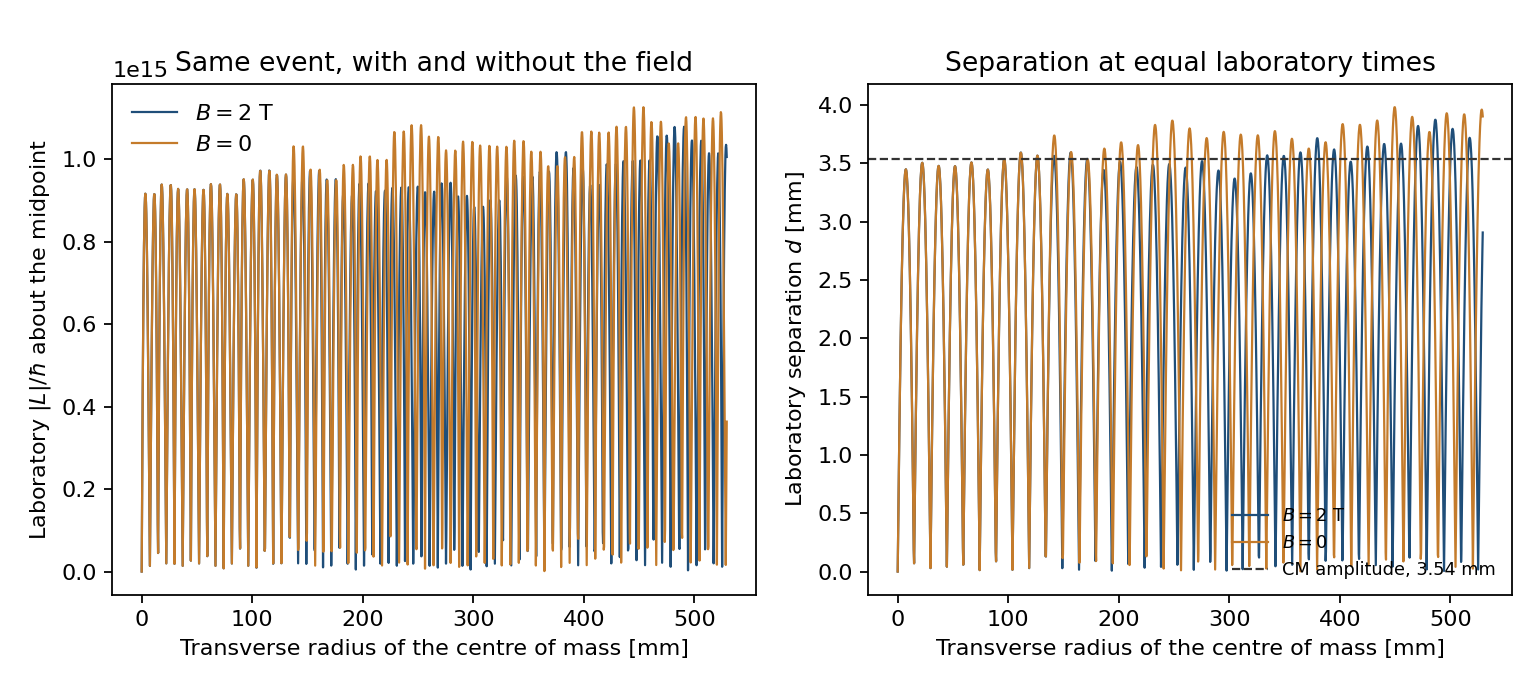
\includegraphics[width=\textwidth]{lab_angular_momentum.png}
\caption{Laboratory angular momentum about the midpoint, and laboratory separation, for the Figure~2 event.
The blue and orange curves are \(B = \SI{2}{\tesla}\) and \(B = 0\).
The dashed line is the centre-of-mass amplitude \(2(\gamma-1)m_Q/\Lambda^{2} = \SI{3.54}{\mm}\).}
\label{fig:Lb}
\end{figure}

\section{Separation and energy}
The amplitude in Eq.~(1) and Eq.~(4) of the paper is the maximum distance of one quirk from the centre of mass,
\[
A = (\gamma-1)\frac{m_Q}{\Lambda^{2}} = \SI{1.769}{\mm}.
\]
The maximum separation of the pair in that frame is \(2A = \SI{3.537}{\mm}\).
The numerical integration with \(\boldsymbol{\beta} = 0\) reaches \(\SI{3.536}{\mm}\).
The value \(\SI{3.874}{\mm}\) quoted for Figure~2 is \(|\mathbf{x}_1-\mathbf{x}_2|\) after the boost, taken at equal laboratory times.
A common laboratory time is not a common centre-of-mass time once \(\boldsymbol{\beta}\neq 0\), so the laboratory distance is not the amplitude in Eq.~(4).
With \(B = 0\) and the same boost, that laboratory maximum is \(\SI{3.981}{\mm}\).

The string direction used by the force is the laboratory separation at that same shared time.
The integrator applies Eq.~(3) of the paper to the laboratory velocities and to that laboratory separation.
In the paper, Eq.~(3) is the straight-string equation in the centre-of-mass frame, where the parallel velocity lies along the displacement at equal centre-of-mass times.

The mechanical energy checked here is
\[
E = E_1 + E_2 + \Lambda^{2}\,|\mathbf{x}_1-\mathbf{x}_2|,
\]
with \(E_i\) the laboratory energy of each quirk and with the separation taken at equal laboratory times.
For a straight string and \(B = 0\), this \(E\) is the conserved energy when the separation is the centre-of-mass separation.
Along each trajectory, \(E\) was sampled at up to 2000 stored steps.
The variation in Table~\ref{tab:L} is \((\max E - \min E)/E_{\mathrm{start}}\).
It is 3.4\% for the at-rest integrations and 6.9\% for the boosted Figure~2 trajectory.
The step is the Runge--Kutta step \(\Delta t = 0.04\, m_Q/\Lambda^{2}\), clipped to the range \(\SI{0.02}{\mm}\)--\(\SI{1}{\mm}\).
The at-rest run already reproduces \(2A\) to a part in a thousand, so this variation is not the origin of the difference between \(\SI{3.54}{\mm}\) and \(\SI{3.87}{\mm}\).
That difference is the difference between the centre-of-mass amplitude and the equal-laboratory-time distance of the boosted pair.

\section{Detector hits}
A hit is recorded at every intersection of a quirk trajectory with one of the eight barrel cylinders, inside the \(|z|\) length of that layer and earlier than \(\SI{25}{\ns}\).
The code does not keep only the first intersection with a layer.
Two intersections of the same layer that are separated by less than \(\SI{1}{\mm}\) of light-travel time are collapsed to one, and hits that fall in the same pixel or a neighbouring pixel are merged.
A later return to the same layer, outside that time gap and outside the pixel neighbourhood, remains a separate hit.

The fiducial requirement follows the paper: after the trigger, each quirk must intersect each of the eight layers at least once, with every retained hit time below \(\SI{25}{\ns}\).
A layer is counted once for this requirement, however many crossings it contains.

The signal region in the paper says that all but one layer must contain 2 hits, and that the remaining layer must contain at least 1 hit.
In the code, ``2 hits'' is implemented as at least two.
A layer with three or more hits satisfies the requirement.
An event fails the pattern only if some layer has no hit, or if two or more layers have fewer than two hits.
Explicitly, with \(n_\ell\) the number of selected hits on layer \(\ell\), the pattern passes when
\[
n_\ell \ge 1 \quad\text{for every layer},
\qquad
\text{and}\qquad
\#\{\ell : n_\ell < 2\} \le 1.
\]

\section{Electroweak reconstruction without the seed prefilter}
The seed prefilter is not part of the paper.
Before the four-hit fit, the code discards a layer-8 pair and a layer-7 pair whose average azimuths differ by more than \(\SI{0.5}{\rad}\) or whose average \(z\) coordinates differ by more than \(\SI{80}{\mm}\).
The paper instead fits every combination of a layer-8 pair and a layer-7 pair that has passed \(\Delta\phi < 0.1\) and \(\Delta z < \SI{2}{\cm}\), and then applies \(\mathbf{x}\cdot\mathbf{n}_3 > 0\), \(\Delta s < \SI{0.05}{\cm}\) and \(\Delta w < \SI{1}{\cm}\).

The same 1040 matched electroweak events, at \(\Lambda = \SI{4}{\keV}\) and with the same per-event resolution seeds, were passed through the plane finder again with that prefilter removed.
The trigger and fiducial counts are unchanged, because the prefilter acts only after both of those requirements.
The reconstruction count rises from 22 to 29.

\begin{table}[H]
\centering
\caption{Electroweak reconstruction efficiency at \(\SI{800}{\GeV}\) and \(\SI{4}{\keV}\). The denominator is the 58 fiducial events. The Wilson interval uses \(z = 1.960\).}
\label{tab:prefilter}
\begin{tabular}{lrrrr}
\toprule
Selection & Count & \(\varepsilon_{\mathrm{reco}}\) & Std.\ error & Wilson 95\% CI \\
\midrule
With the seed prefilter    & \(22/58\) & 0.379 & 0.064 & [0.266, 0.508] \\
Without the seed prefilter & \(29/58\) & 0.500 & 0.066 & [0.375, 0.625] \\
\bottomrule
\end{tabular}
\end{table}

Removing the prefilter recovers seven events that pass \(\Delta s < \SI{0.01}{\cm}\), \(\Delta w < \SI{1}{\cm}\), and the hit pattern.
The prefilter is therefore not equivalent to the paper's width cut: it rejects events that later satisfy the signal region.
The Table~I value 0.72 lies outside both intervals.
The trigger efficiency of this sample remains \(182/1040 = 0.175\), and the fiducial efficiency remains \(58/182 = 0.319\).

\section{Colored benchmark at \(\Lambda = \SI{2}{\keV}\)}
Figure~5 and Table~I of the paper use \(\Lambda = \SI{2}{\keV}\) for the colored benchmark, with \(m_Q = \SI{1800}{\GeV}\).
The 855 events already matched by MadGraph and Pythia were propagated again at this string scale.
The hard-process momenta, the resolution seeds, the seed prefilter, and the charges are those of the \(\SI{4}{\keV}\) colored run.
Only \(\Lambda\) was changed.
Table~I gives \(\varepsilon_{\mathrm{reco}} = 0.35\) at \(\SI{2}{\keV}\), \(0.59\) at \(\SI{3}{\keV}\), and \(0.74\) at \(\SI{5}{\keV}\).
It gives \(\varepsilon_{\mathrm{trig}} = 0.24\) and \(\varepsilon_{\mathrm{fid}} = 0.28\), both independent of \(\Lambda\) apart from small edge effects in the fiducial efficiency.

\begin{table}[H]
\centering
\caption{Colored efficiencies from the same 855 matched events. The \(\SI{4}{\keV}\) row is the run already reported. The \(\SI{2}{\keV}\) row is the new propagation.}
\label{tab:qcd2}
\small
\begin{tabular}{llrrrr}
\toprule
\(\Lambda\) & Efficiency & Count & Estimate & Std.\ error & Wilson 95\% CI \\
\midrule
\SI{2}{\keV} & \(\varepsilon_{\mathrm{trig}}\) & \(208/855\) & 0.243 & 0.015 & [0.216, 0.273] \\
\SI{2}{\keV} & \(\varepsilon_{\mathrm{fid}}\)  & \(54/208\)  & 0.260 & 0.030 & [0.205, 0.323] \\
\SI{2}{\keV} & \(\varepsilon_{\mathrm{reco}}\) & \(34/54\)   & 0.630 & 0.066 & [0.496, 0.746] \\
\midrule
\SI{4}{\keV} & \(\varepsilon_{\mathrm{trig}}\) & \(208/855\) & 0.243 & 0.015 & [0.216, 0.273] \\
\SI{4}{\keV} & \(\varepsilon_{\mathrm{fid}}\)  & \(54/208\)  & 0.260 & 0.030 & [0.205, 0.323] \\
\SI{4}{\keV} & \(\varepsilon_{\mathrm{reco}}\) & \(29/54\)   & 0.537 & 0.068 & [0.406, 0.663] \\
\bottomrule
\end{tabular}
\end{table}

The trigger count is fixed by the generated \(p_T\) and does not depend on \(\Lambda\).
The fiducial count is also unchanged between these two string scales: 54 events at both \(\SI{2}{\keV}\) and \(\SI{4}{\keV}\).
The reconstruction efficiency rises from 0.537 at \(\SI{4}{\keV}\) to 0.630 at \(\SI{2}{\keV}\).
The Table~I entry 0.35 lies outside the Wilson interval \([0.496, 0.746]\).

\section{Charge in the colored force}
The Lorentz force is \(q\,\mathbf{v}\times\mathbf{B}\), with the charge taken from the particle in the MadGraph event.
For the colored sample that particle is the vector-like quark \texttt{tp}, PDG code 6000006, and the charge stored on the trajectory is \(+2/3\) for \texttt{tp} and \(-2/3\) for \(\bar t'\).
The \(\SI{2}{\keV}\) run in Table~\ref{tab:qcd2} uses these same charges.

The paper lets the colored quirks hadronize.
The charged quirk-hadrons are then taken to have charge \(\pm 1\), and the probability of that charged outcome is given as about 30\%.
The paper states that the tracking study depends on the charges being nonzero, rather than on their exact values.
In this implementation the 30\% factor is not applied inside \(\varepsilon_{\mathrm{trig}}\), \(\varepsilon_{\mathrm{fid}}\), or \(\varepsilon_{\mathrm{reco}}\).
The force law itself uses \(\pm 2/3\), not \(\pm 1\).
The electroweak trajectory uses charge \(\pm 1\), which is the unit charge of the vector-like lepton.

\end{document}
